\section*{Lectura 6: La Teoreman Fundamental del Algebra.}

\begin{theorem}[La Teorema Fundamental del Algebra]\label{thm_6.11}
    Todo polinomio con coeficientes complejas tiene al menos una ra\'iz
    complejo.
\end{theorem}
\begin{proof}
    Sea $\Sigma_\rho \subseteq \C$ el circulo de radio  $\rho$ en  $\C$.
    Considere la mapa  $f:\C \xrightarrow{} \C$ dado por $f(z)=z^n$, y denota
    $f^n_\rho=f|_{\Sigma_\rho}$. Nota que los $f^n_\rho$ son homotopicamentes
    nulas.

    Ahora, considere el polinomio  $g(z)=z^n+a_{n-1}z^{n-1}+\dots+a_1z+a_0$
    donde $a_i \in \C$ para todo  $0 \leq i \leq n$ y  $\deg{g}=n \geq 1$.
    Escoga $\rho>\max{\{1,\sum{|a_i|}\}}$, y defina la mapa $F:\Sigma_\rho
    \times I \xrightarrow{} \C$ dado por
    \begin{equation*}
        F(z,t)=z^n+\sum_{i=0}^{n-1}{(1-t)a_iz^i}
    \end{equation*}
    Por la contunuidad de polinomios en $\C$, tenemos que  $F$ es continua. Mas
    a\'un tenemos que  $F(z,0)=z^n+a_{n-1}z^{n-1}+\dots+a_1z_1+a_0=g(z)$ y
    $F(z,1)=z^n=f^n_\rho$. As\'i que $f^n_\rho \simeq g$ son homotopicos atraves
    de la homotopia $F$.

    Afirmamos que $F(z,t) \neq 0$. Por lo contrario, asuma que existe un $(z,t)
    \in \Sigma_\rho \times I$ tal que $F(z,t)=0$. Entonces tenemos que
    \begin{equation*}
        z^n=-\sum_{i=0}^{n-1}{(1-t)a_iz^i}
    \end{equation*}
    Por la desigualdad de triangulo, tenemos
    \begin{equation*}
        |z^n|=\rho^n \leq \sum{(1-t)|a_i|\rho^i} \leq \rho^{n-1}\sum{(1-t)|a_i|}
    \end{equation*}
    como $\rho>1$ y  $t \in I$ implica que  $\sum{(1-t)|a_i|} \leq \sum{|a_|}$,
    tenemos que
    \begin{equation*}
        \rho \leq \sum_{i=0}^{n-1}{(1-t)|a_i|}
    \end{equation*}
    lo cual contradice neustor escojido de $\rho$. Asi que  $F(z,t) \neq 0$ para
    todos $(z,t) \in \Sigma_\rho \times I$.

    \begin{figure}[h]
        \centering
        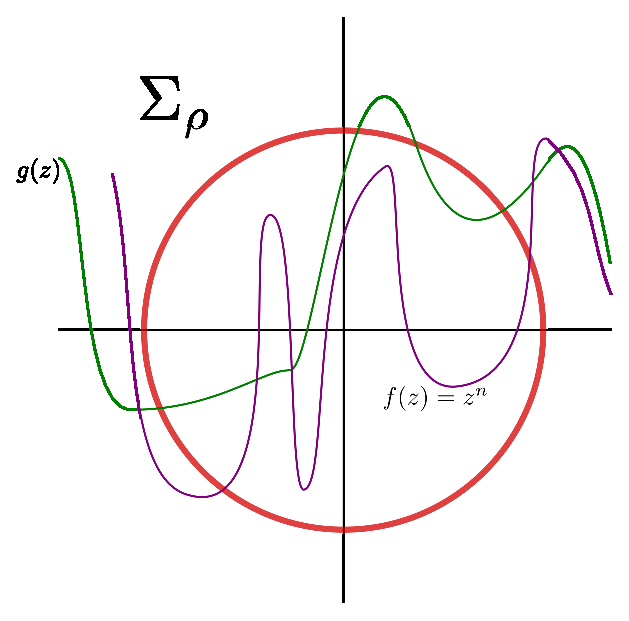
\includegraphics[scale=0.5]{Figures/fund_thm_algebra.eps}
        \caption{La teorema Fundamental del Algebra. Nota que $f^n_\rho$ consiste de
        cuyas puntos de $f(z)=z^n$ cuyas puntos intersecan con $\Sigma_\rho$.}
        \label{fig_16}
    \end{figure}

    Finalmente, tenemos que $F:\Sigma_\rho \times I \xrightarrow{}
    \com{\C}{\{0\}}$. Entonces suponga que $g(z)$ no tiene raices complejas.
    Defina $G:\Sigma_\rho \times I \xrightarrow{} \com{\C}{\{0\}}$ dado por
    $G(z,t)=g((1-t)z)$. Tenemos que $(1-t)z$ es una mapa continua, y que $g$ es
    continua; por lo tanto por composici\'on,  $G$ tambien es continua  (de
    hecho, es continua en $z$ y en  $t$). Mas a\'un, tenemos $G(z,0)=g(z)$ y
    $G(z,1)=g(0)=a_0$. As\'i que $g$ es homotopica a la mapa constante  $k:z
    \xrightarrow{} a_0$, por lo tanto es homotopicamente nula. Por transitividad
    de homotopia, $f^n_\rho$ tambien es homotopicamente nula, lo cual es
    imposible. Por lo tanto,  $g$ tiene que tener al menos una raiz en $\C$.
\end{proof}
